\section{Evaluation}
\label{section:evaluation}
Evaluation of the GearSmarts API was done via Node.js scripts automating the training and classifying of files
stored on the filesystme. Evaluation was done in two main parts: first evaluating GearSmarts against known, large datasets
to verify the machine learning core works well and as expected, and second evaluating GearSmarts with the collected
outfit-comfort responses.

Evaluations of the classifier are recorded in terms of ``True Positive" (TP), ``False Negative" (FN), ``False Positive"
(FP), \& ``True Negative" (TN), indicating what was predicted verse what the data's actual class. Then, the results are
presented in terms of some commonly used formulas: ``Precision", ``Recall", ``Specificity", and ``Accuracy"
\cite{measures}. A description of these formulas is shown in table \ref{table:measures}.

In the case of datasets with more than 2 classes, such as the outfit comfort survey, the measurements are made once for
each of the classes. This shows the performance of the classifier on each class versus all the rest.

\begin{table}
    \begin{tabular}{lll}
        \hline
        \textbf{Measure} & \textbf{Formula} & \textbf{Meaning} \\ [0.5ex]
        \hline\hline
        Precision	& TP / (TP + FP) & \% of correct +'s \\
        Accuracy	& (TP + TN) / (total) & \% correct \\
        Recall 	    & TP / (TP + FN) & \% of +'s predicted as + \\
        Specificity	& TN / (TN + FP) & \% of -'s predicted as + \\
        \hline
    \end{tabular}
    \caption{The measurement terms used in evaluations for this project, with their formulas and intuitive meanings}
    \label{table:measures}
\end{table}

\subsection{Public Datasets}
\label{subsection:publicdatasets}
First, to evaluate the efficacy of the machine learning core, GearSmarts was evaluated using datasets from LIBSVM \cite{libsvm:datasets}.
A large part of the evaluation was the question of how would the feature and classification dictionary and indexing implementation
impact performance.

A Node.js script was used to parse train and test files, query the GearSmarts API with each, and evaluate the performance.
The evaluation script and datasets can be found in the \texttt{eval/} directory of the source code for this report.
Three public datasets were evaluated: ``a1a'', ``a2a'', and ``a3a'', all with decent results, shown in figure \ref{fig:aXa}.
The datasets have 1,605/30,956, 2,265/30,296, and 3,185/29,376 training/testing datapoints each, respectively.

\begin{figure}[ht!]
    \centering
    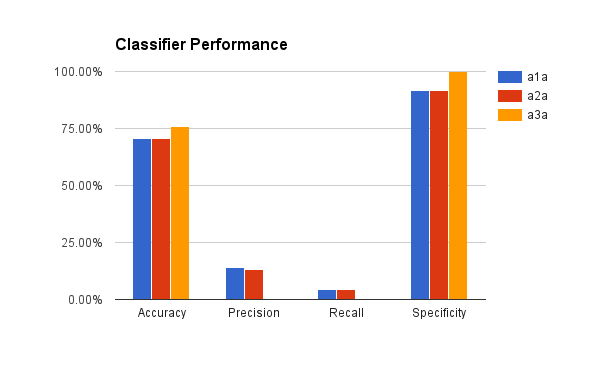
\includegraphics[width=90mm]{img/aXa.png}
    \caption{GearSmarts classifier performance on the aXa datasets}
    \label{fig:aXa}
\end{figure}

\subsection{Outfit Comfort}
TODO

\subsubsection{Pre-processing}
\label{subsection:preprocessing}

TODO